\documentclass{beamer}
\usepackage{graphicx}
\usepackage[slovene]{babel}
\usepackage[utf8]{inputenc}

\usepackage{gensymb}
\usepackage{xcolor}

\setlength{\parindent}{0em}
\setlength{\parskip}{-1em} 

\definecolor{labitorange}{RGB}{200, 0, 0}
\usetheme{Singapore}
\usecolortheme{dove}
\setbeamercolor*{structure}{fg=labitorange!100}

\title{Celtrin programerski izziv: Operacija Periskop}
\author{Andrej Dolenc}
\institute{\small{FMF IŠRM II}}
\date{\small{\today}}

% Remove navigation symbols
\setbeamertemplate{navigation symbols}{}

% % Show overview at every subsection
% \AtBeginSubsection[]
% {
%   \begin{frame}<beamer>
%     \frametitle{Outline}
%     \tableofcontents[
%       currentsection,
%       sectionstyle=show/show,
%       subsectionstyle=show/shaded/hide]
%   \end{frame}
% }

% Hide navigation header
\makeatletter
\renewcommand*\insertnavigation[1]{\vspace{16pt}}
\makeatother

\usepackage{textcomp}
\usepackage{tikz}
\usetikzlibrary{calc}

\makeatletter
\def\progressbar@progressbar{}
\newcount\progressbar@tmpcounta
\newcount\progressbar@tmpcountb
\newdimen\progressbar@pbht
\newdimen\progressbar@pbwd
\newdimen\progressbar@tmpdim

\progressbar@pbwd=\paperwidth
\progressbar@pbht=2pt

% the progress bar
\def\progressbar@progressbar{%

    \progressbar@tmpcounta=\insertframenumber
    \progressbar@tmpcountb=\inserttotalframenumber
    \advance \progressbar@tmpcounta by -1
    \advance \progressbar@tmpcountb by -1
    % \advance \progressbar@tmpcounta by -2
    % \advance \progressbar@tmpcountb by -2
    \progressbar@tmpdim=\progressbar@pbwd
    \multiply\progressbar@tmpdim by \progressbar@tmpcounta
    \divide\progressbar@tmpdim by \progressbar@tmpcountb

  \begin{tikzpicture}

      % slider
    \usebeamercolor{normal text}
    \fill[color=bg!90!fg]
      (0pt, 0pt) rectangle ++ (\progressbar@pbwd, \progressbar@pbht);

    \usebeamercolor{structure}
    \fill[color=fg!75!bg]
      (0pt, 0pt) rectangle ++ (\progressbar@tmpdim, \progressbar@pbht);

      % page number
    \usebeamercolor{normal text}
    \node[color=fg, align=center, anchor=east] at
    (\progressbar@pbwd, \progressbar@pbht * 4) {\insertframenumber /\inserttotalframenumber};

      % title
    % \node[color=fg, align=center, anchor=west] at
    % (0, \progressbar@pbht * 4) {\footnotesize{\insertauthor}};
  \end{tikzpicture}
}

% \addtobeamertemplate{footline}{}
% {
%   % Show progressbar
%   \progressbar@progressbar
% }
% \makeatother


\begin{document}

% Title frame
{
  % Hide progressbar from frame
  \setbeamertemplate{footline}{} 
  % Hide navigation bar from frame
  \renewcommand*\insertnavigation[1]{\vspace{22pt}}
  \begin{frame}
    \vspace{60pt}
    \titlepage
  \end{frame}
}
% % Don't count title frame as a frame
% \addtocounter{framenumber}{-1}

% % Outline frame
% {
% \renewcommand*\insertnavigation[1]{\vspace{22pt}}
% \begin{frame}{Kazalo}
%   \tableofcontents
% \end{frame}
% }

\begin{frame}{Opis naloge}
  \begin{tikzpicture}[remember picture,overlay]
      \node[xshift=-2.7cm,yshift=3.6cm] at (current page.south east) {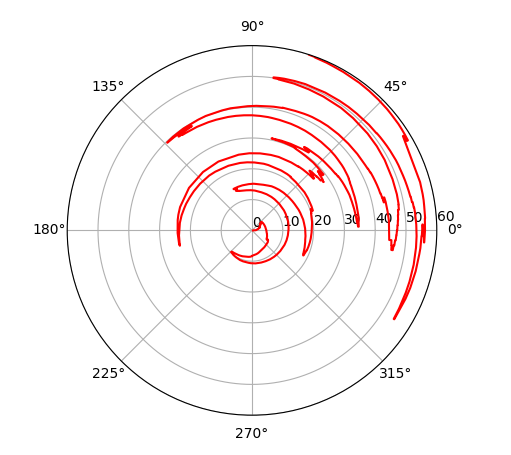
\includegraphics[width=6.0cm]{img/trace.png}};
  \end{tikzpicture}
  \vspace{-60pt}
  \begin{itemize}
    \item $360\degree$ video
    \item Učni podatki: 86 sledi pogledov uporabnikov
    \item Testni podatki
    \begin{itemize}
      \item $4s$ znanih kotov
      \item $4s$ neznanih kotov
    \end{itemize}
    \item Katere tokove naložiti v \\ predpomnilnik uporabnika?
  \end{itemize}
\end{frame}

\begin{frame}{Smiselna delitev naloge}
  \begin{itemize}
    \item Določanje kotov pogleda uporabnikov za $4$ neznane sekunde
    \item Določanje tokov ki jih pošljemo uporabniku
  \end{itemize}
\end{frame}

\begin{frame}{Analiza podatkov: vročinska slika}
  \begin{figure}
    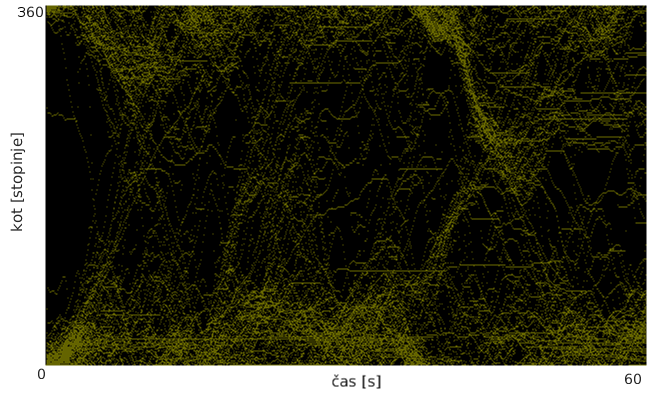
\includegraphics[scale=0.67]{img/hm-kd.png}
  \end{figure}
\end{frame}

\begin{frame}{Pomembnosti stolpcev v zornem kotu}
  \begin{tikzpicture}[remember picture,overlay]
      \node[xshift=6.3cm,yshift=0cm] at (current page.west) {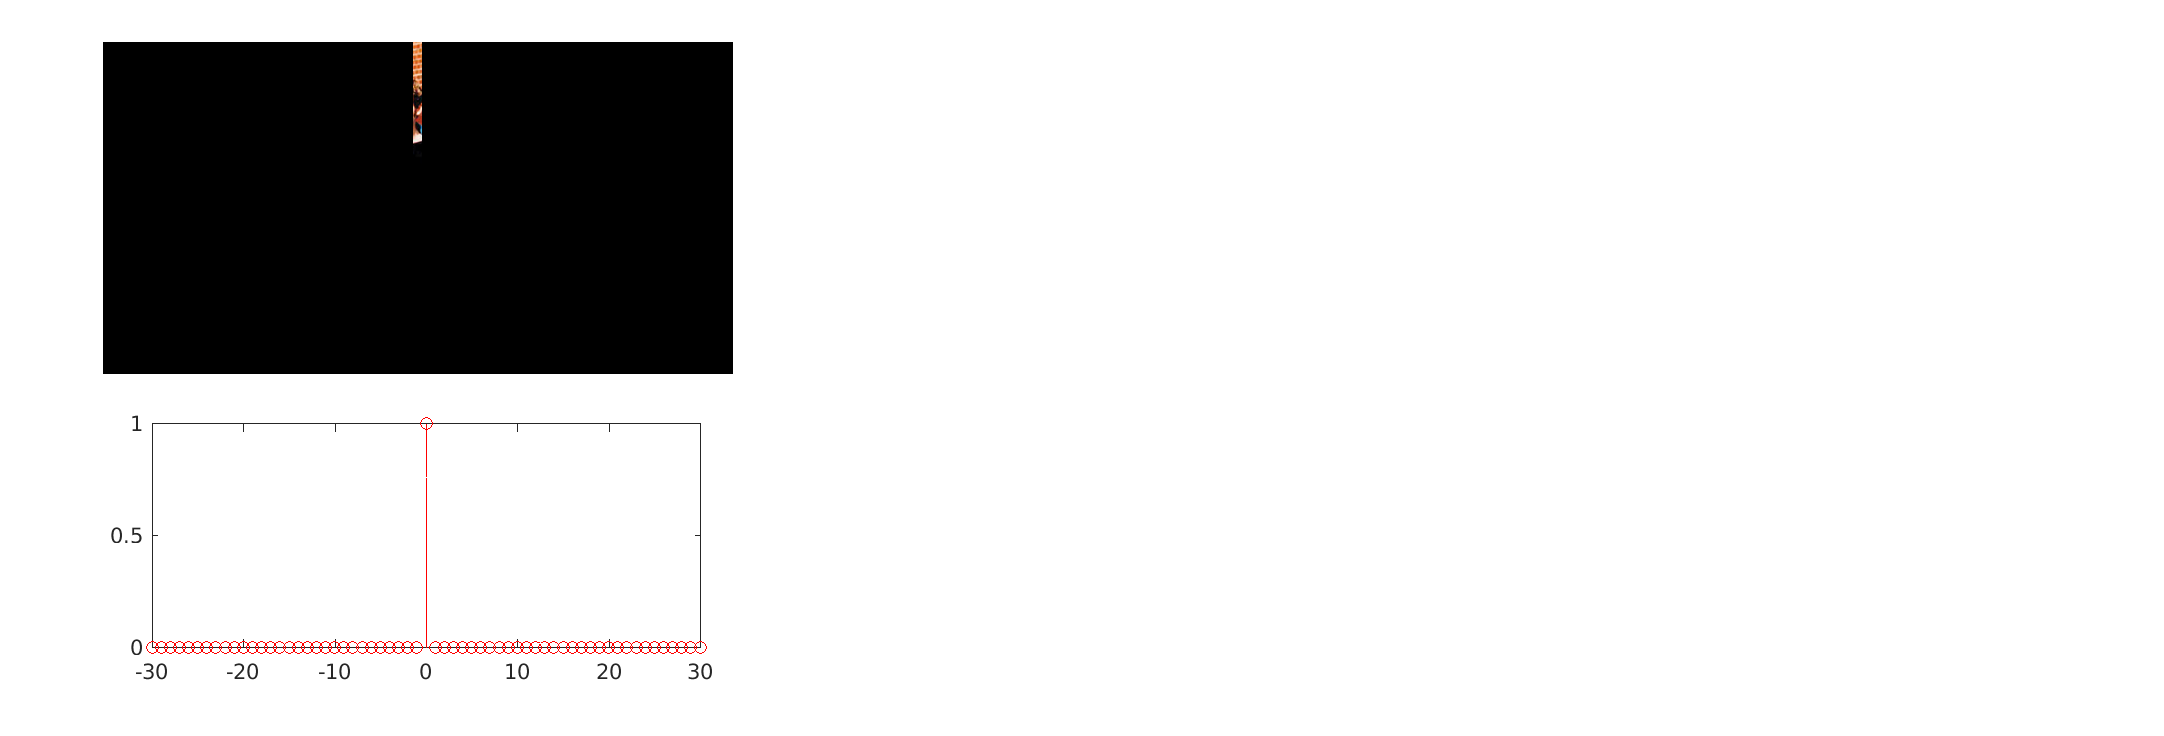
\includegraphics[width=12.0cm]{img/views1.png}};
  \end{tikzpicture}
\end{frame}

\begin{frame}{Pomembnosti stolpcev v zornem kotu}
  \begin{tikzpicture}[remember picture,overlay]
      \node[xshift=6.3cm,yshift=0cm] at (current page.west) {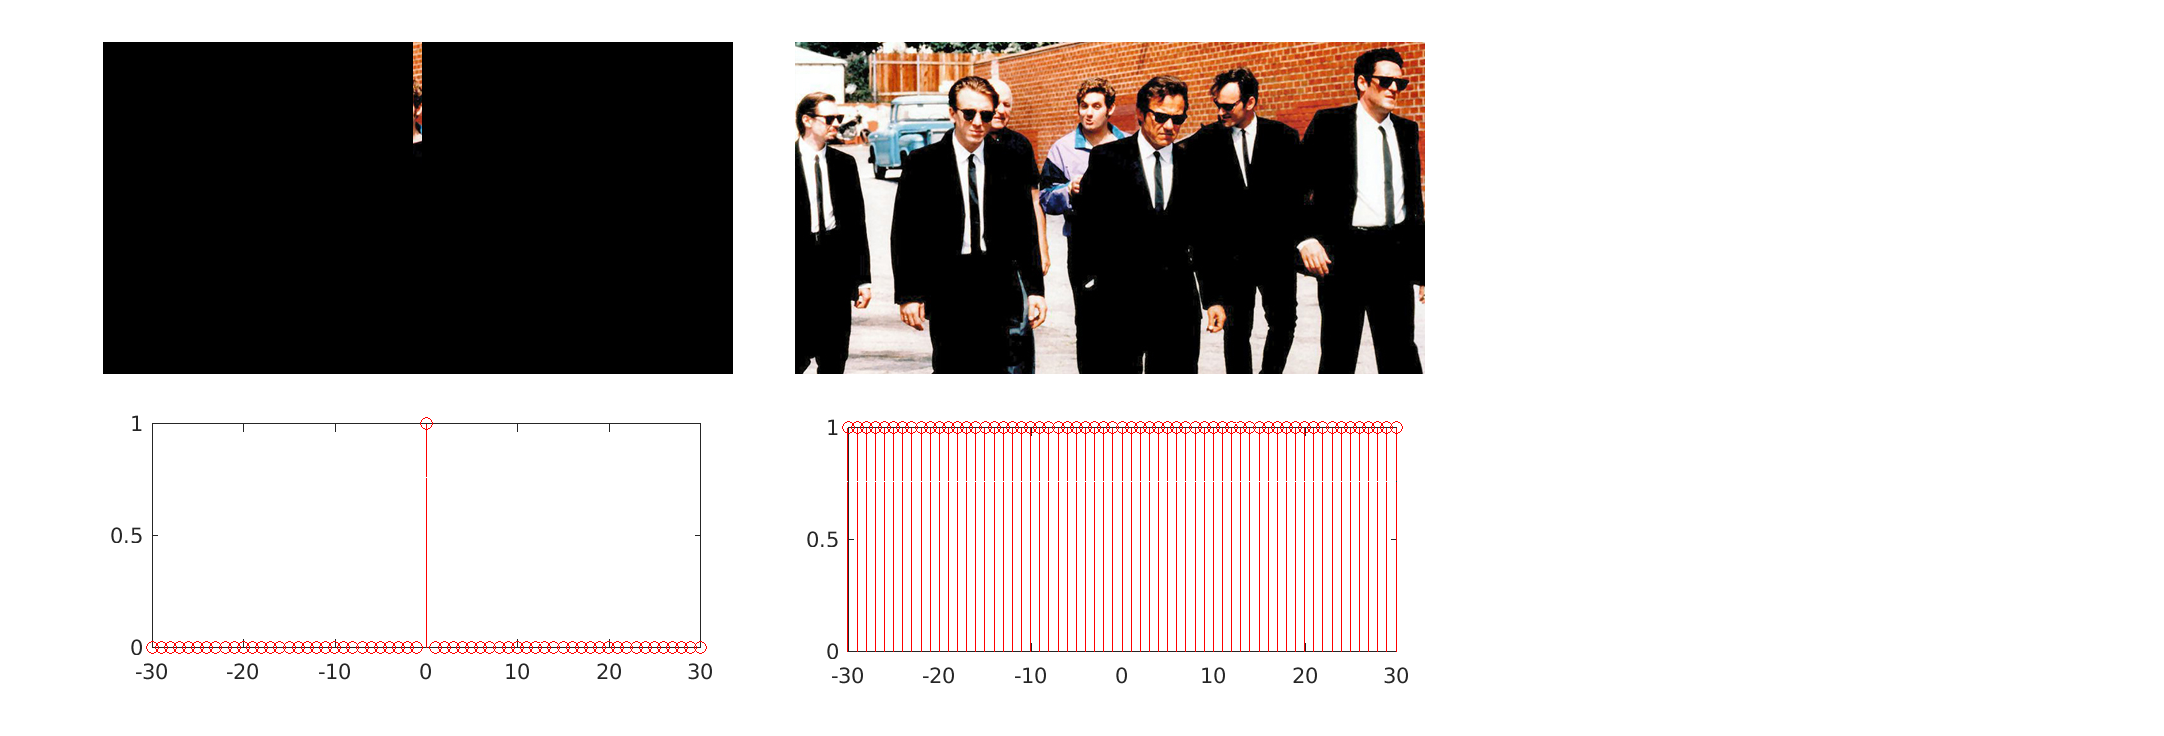
\includegraphics[width=12.0cm]{img/views2.png}};
  \end{tikzpicture}
\end{frame}

\begin{frame}{Pomembnosti stolpcev v zornem kotu}
  \begin{tikzpicture}[remember picture,overlay]
      \node[xshift=6.3cm,yshift=0cm] at (current page.west) {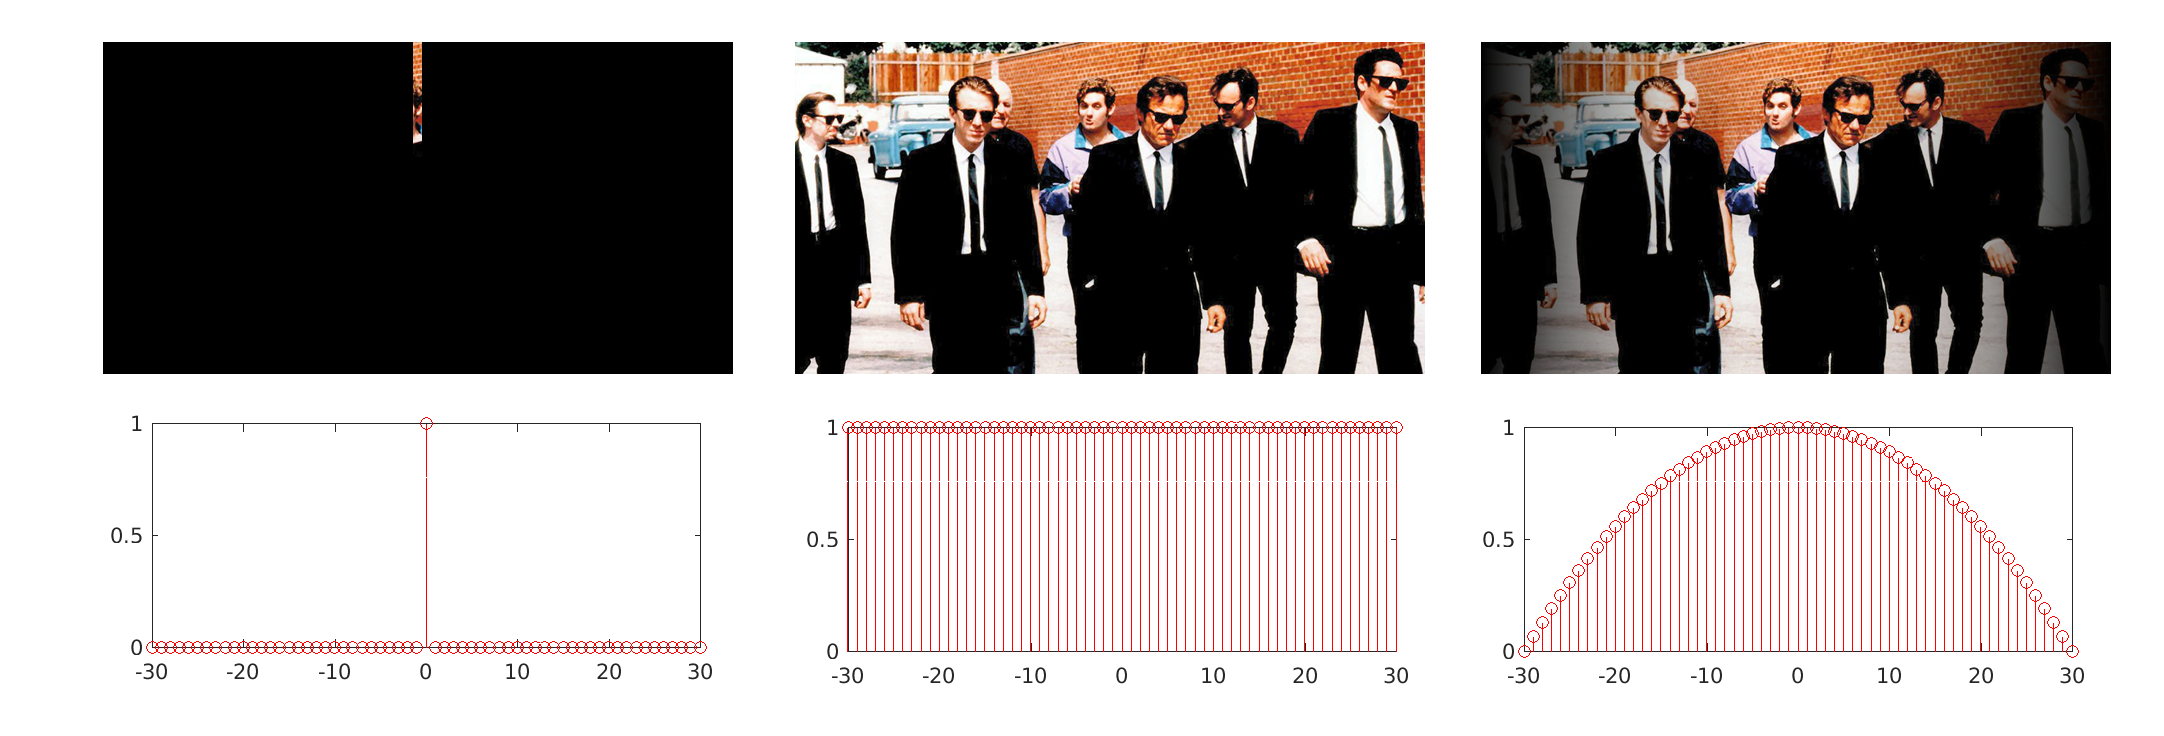
\includegraphics[width=12.0cm]{img/views3.png}};
  \end{tikzpicture}
\end{frame}

\begin{frame}{Vročinska slika z Welch oknom}
  \begin{figure}
    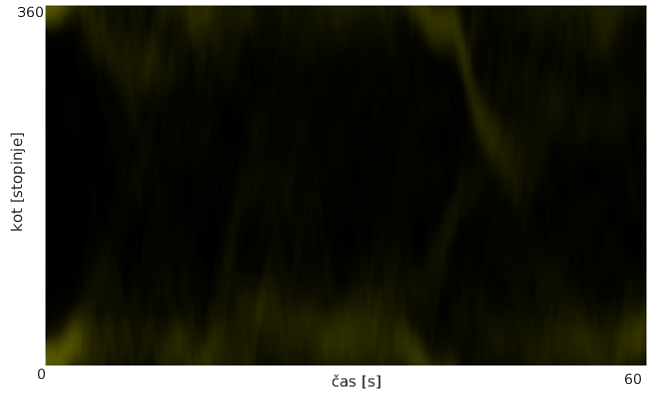
\includegraphics[scale=0.67]{img/hm-we.png}
  \end{figure}
\end{frame}

\begin{frame}{Vročinska slika z Welch oknom}
  \begin{figure}
    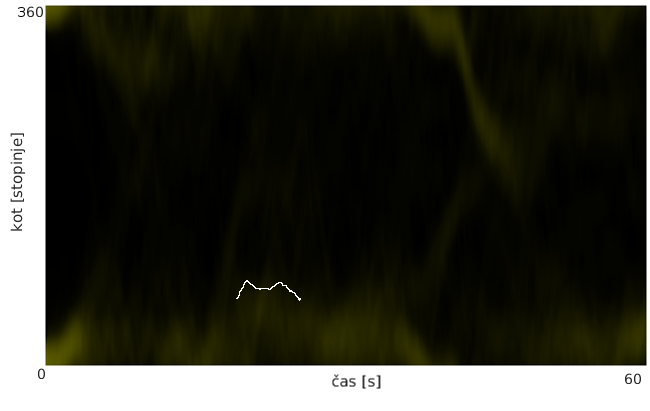
\includegraphics[scale=0.67]{img/hm-wet.png}
  \end{figure}
\end{frame}

\begin{frame}{Maksimiziranje rumene barve}
  \begin{itemize}
    \item Z uporabo dinamičnega programiranja
  \end{itemize}

\begin{displaymath}
  sc(\theta, t) = heatmap(\theta, t) + \left\{ \begin{array}{ll}
                                            0 & \textrm{če $t = 60$,}\\
                                            \displaystyle \max_{\theta'}\{w(\theta'-\theta) \cdot sc(\theta', t+1)\} & \textrm{sicer.}
  \end{array} \right.
\end{displaymath}
  \begin{figure}
    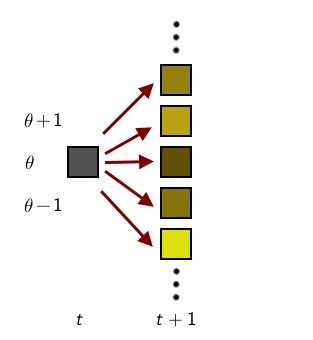
\includegraphics[scale=0.57]{img/dp.png}
  \end{figure}
\end{frame}

\begin{frame}{Maksimiziranje rumene barve}
  \begin{itemize}
    \item Z uporabo dinamičnega programiranja
  \end{itemize}

\begin{displaymath}
  sc(\theta, t) = heatmap(\theta, t) + \left\{ \begin{array}{ll}
                                            0 & \textrm{če $t = 60$,}\\
                                            \displaystyle \max_{\theta'}\{w(\theta'-\theta) \cdot sc(\theta', t+1)\} & \textrm{sicer.}
  \end{array} \right.
\end{displaymath}
  \begin{figure}
    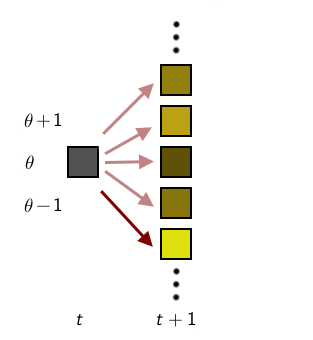
\includegraphics[scale=0.57]{img/dp2.png}
  \end{figure}
\end{frame}

\begin{frame}{Analiza podatkov: relativni premiki uporabnikov}
  \begin{figure}
    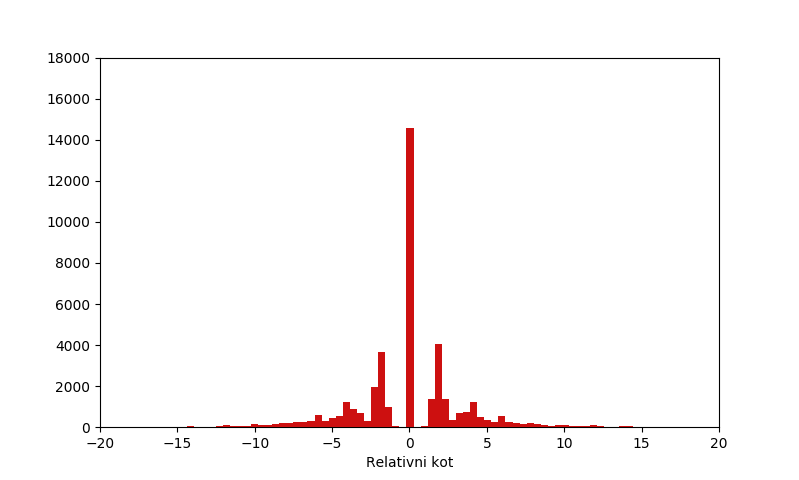
\includegraphics[scale=0.55]{img/rel_moves.png}
  \end{figure}
\end{frame}

\begin{frame}{Maksimiziranje rumene barve}
  \begin{itemize}
    \item Z uporabo dinamičnega programiranja
  \end{itemize}

\begin{displaymath}
  sc(\theta, t) = heatmap(\theta, t) + \left\{ \begin{array}{ll}
                                            0 & \textrm{če $t = 60$,}\\
                                            \displaystyle \max_{\theta'}\{w(\theta'-\theta) \cdot sc(\theta', t+1)\} & \textrm{sicer.}
  \end{array} \right.
\end{displaymath}
  \begin{figure}
    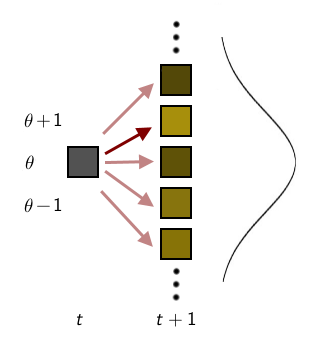
\includegraphics[scale=0.57]{img/dp3.png}
  \end{figure}
\end{frame}

\begin{frame}{Razbitje videa na tokove}
  \begin{itemize}
    \item Izhodišče: želimo zagotoviti optimalno kvaliteto za znane 4 sekunde
  \end{itemize}
\end{frame}

\begin{frame}{Razbitje videa na tokove}
  \begin{itemize}
    \item 90 tokov po $4\degree$ kvalitete $100\%$
    \item 1 tok $360\degree$ kvalitete $1\%$
    \item Želimo čim pokriti čim več kotov na vsako stran
  \end{itemize}
  \begin{figure}
    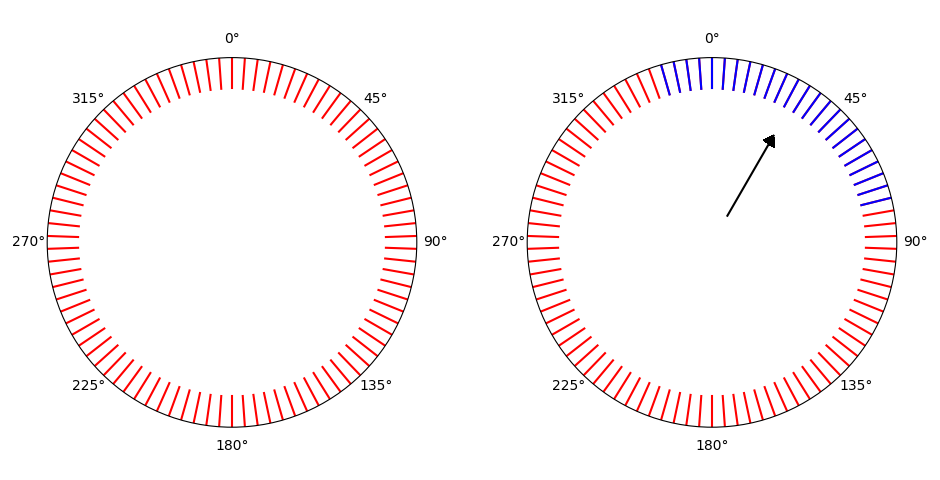
\includegraphics[scale=0.4]{img/streams.png}
  \end{figure}
\end{frame}

\begin{frame}{Nastavljanje parametrov}
  \begin{itemize}
    \item Parametri:
    \begin{itemize}
      \item Resolucija vročinske slike
      \item Okno pri vročinski sliki
      \item Uteži pri DP
      \item Različne strategije za tokove
    \end{itemize}
    \item Nastavimo s pomočjo prečnega preverjanja
  \end{itemize}
\end{frame}

\begin{frame}{Problemi}
  \begin{itemize}
    \item DP ne da nujno optimalne poti
    \item Če uporabniku preveč napačno napovemo kot, bo gledal kvaliteto $1\%$
    \item \ldots
  \end{itemize}
\end{frame}

\begin{frame}{}
  \centering
  \huge{Vprašanja?}
\end{frame}


\end{document}
